\documentclass{article}

\usepackage[left = 3cm, right = 3cm, top = 3cm]{geometry}
\usepackage{tikz}
\usepackage{amsmath}
\usepackage{amssymb}
\usepackage{graphicx}
\usepackage{mathtools}

\DeclarePairedDelimiter{\norm}{\lVert}{\rVert}
\newcommand{\R}{\mathbb{R}}

\graphicspath{{./}}

\title{Project Report}
\author{Hao Gao, Trisha Trupng, Karen Hovhannisyan, Chenhao Li, ZiYao Cui}
\date{December 1, 2018}


\begin{document}
\maketitle 
\section*{General Background}
We decided to do our project on housing prices. Buying a house is a big event for anybody and a home is usually ones biggest asset in life. Therefore, trying to find a house that fits one’s needs and wants but also is within budget, is a problem that begs for a solution. It is also important to be able to calculate the sale price of a home based on certain features, so that buyers can know the cost of their desired attributes. Because a sale price is a reflection of all aspects of the house it is hard to discern at first glance how significant the various factors are. Creating a regression model to achieve this insight would surely be useful for home buyers and the real estate world so they can forecast the market. It is also important for students our age to know this because of how soon we will be entering the real world and looking for houses of our own. 
\section*{Data Outline}
Our dataset contains about 2274 observations of housing price with at first 28 explanatory variables describing the aspect of the house. Those variables include:\\
\textbf{Lotfront}: Linear feet of street connected to property\\
\textbf{Lotarea}: Lot size in square feet\\
\textbf{YearBuilt}: The year the house was built\\
\textbf{YearRemodADD}: The year the house was remoded\\
\textbf{MasVnrArea}: Masonry veneer area in square feet\\
\textbf{BsmtFinSF1}: Type 1 finished square feet\\
\textbf{BsmtFinSF2}: Type 2 finished square feet\\
.\\
.\\
.\\
\textbf{Age}: The house age\\
\textbf{Agerem}:  Age of the house since re modeled\\
\textbf{Sf}: Total square footage\\
\textbf{Fsf}: First floor square footage\\
\textbf{Ssf}: Second floor square footage\\
\textbf{Bath}: Number of Bathroom\\
\textbf{Bedroom}: Number of Bedroom\\
\textbf{Garage}: Size of garage in square feet\\
The original data set came from Ames, Iowa where the Assessor’s office of the city compiled date from all house sales in the city between 2006 and 2010, with 2930 observations and 80 different variables. We removed most of the discrete variables from the data set and considered the ones that seemed to be the most important. We also delete all samples those contains missing values, such as thosw with "NA" or "None" in the predictor entries. 

\section*{Linear Regression Model}
At first we applied the first order linear model to fit our data set: \\
$\hat{Y_i} = \textbf{X}\textbf{B}$\\
where $\textbf{B} = $ $\begin{pmatrix} \beta_1 \\ \beta_2 \\ ... \\ \beta_{28} \end{pmatrix}$, $\textbf{X} = $ $\begin{pmatrix}X_{i1} \\ X_{i2} \\... \\  X_{i3} \\ X_{i28} \end{pmatrix}$. 
In the model selection and interpretation step, we will drop certain predictors that might have zero coefficients and seek the influence of iteractions.\\
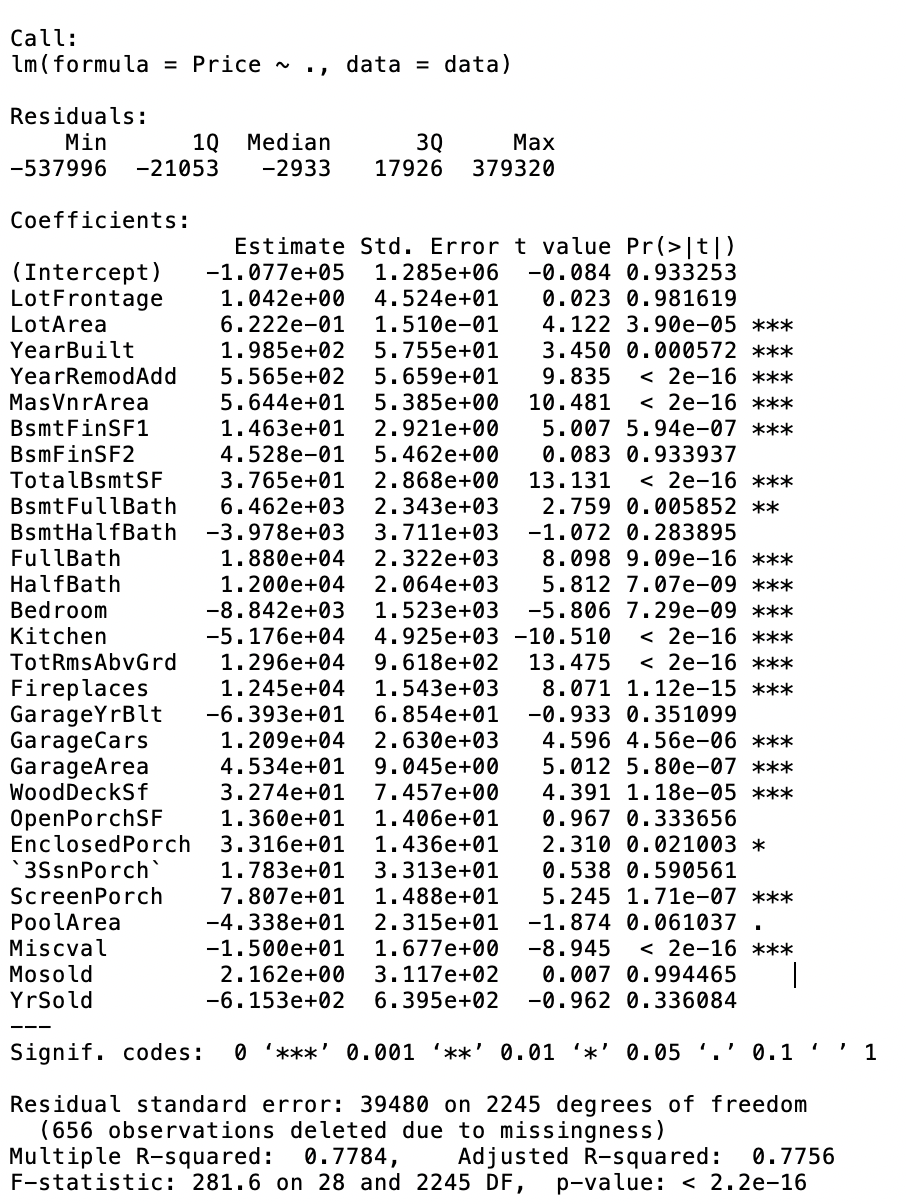
\includegraphics[scale = 0.5]{reg1.png}\\
% $\hat{Y_i}=(1.19 \times 10^2) X_{i1} + (1.65 \times 10^0) X_{i2} - (5.71\times 10^2) X_{i3} - (5.44 \times 10^2) X_{i4} + (6.06 \times 10) X_{i5} +(7.09 \times 10) X_{i6} + (9.72 \times 10) X_{i7} - (1.06 10^4) X_{i8} - (1.71 \times 10^4) X_{i9} + (4.73 \times 10^4) X_{i10} + 6.667 \times 10^4$


\section*{Assumtions}
We assume that there exist a linear relashionship along the response variable "Price" and all other predictor variables. We also hope the residuals has constance variance. To check for such two assumptions, we plot residuals agains response variable, as well as residuals against some other variables in our model. Here are 11 of residual plots: \\
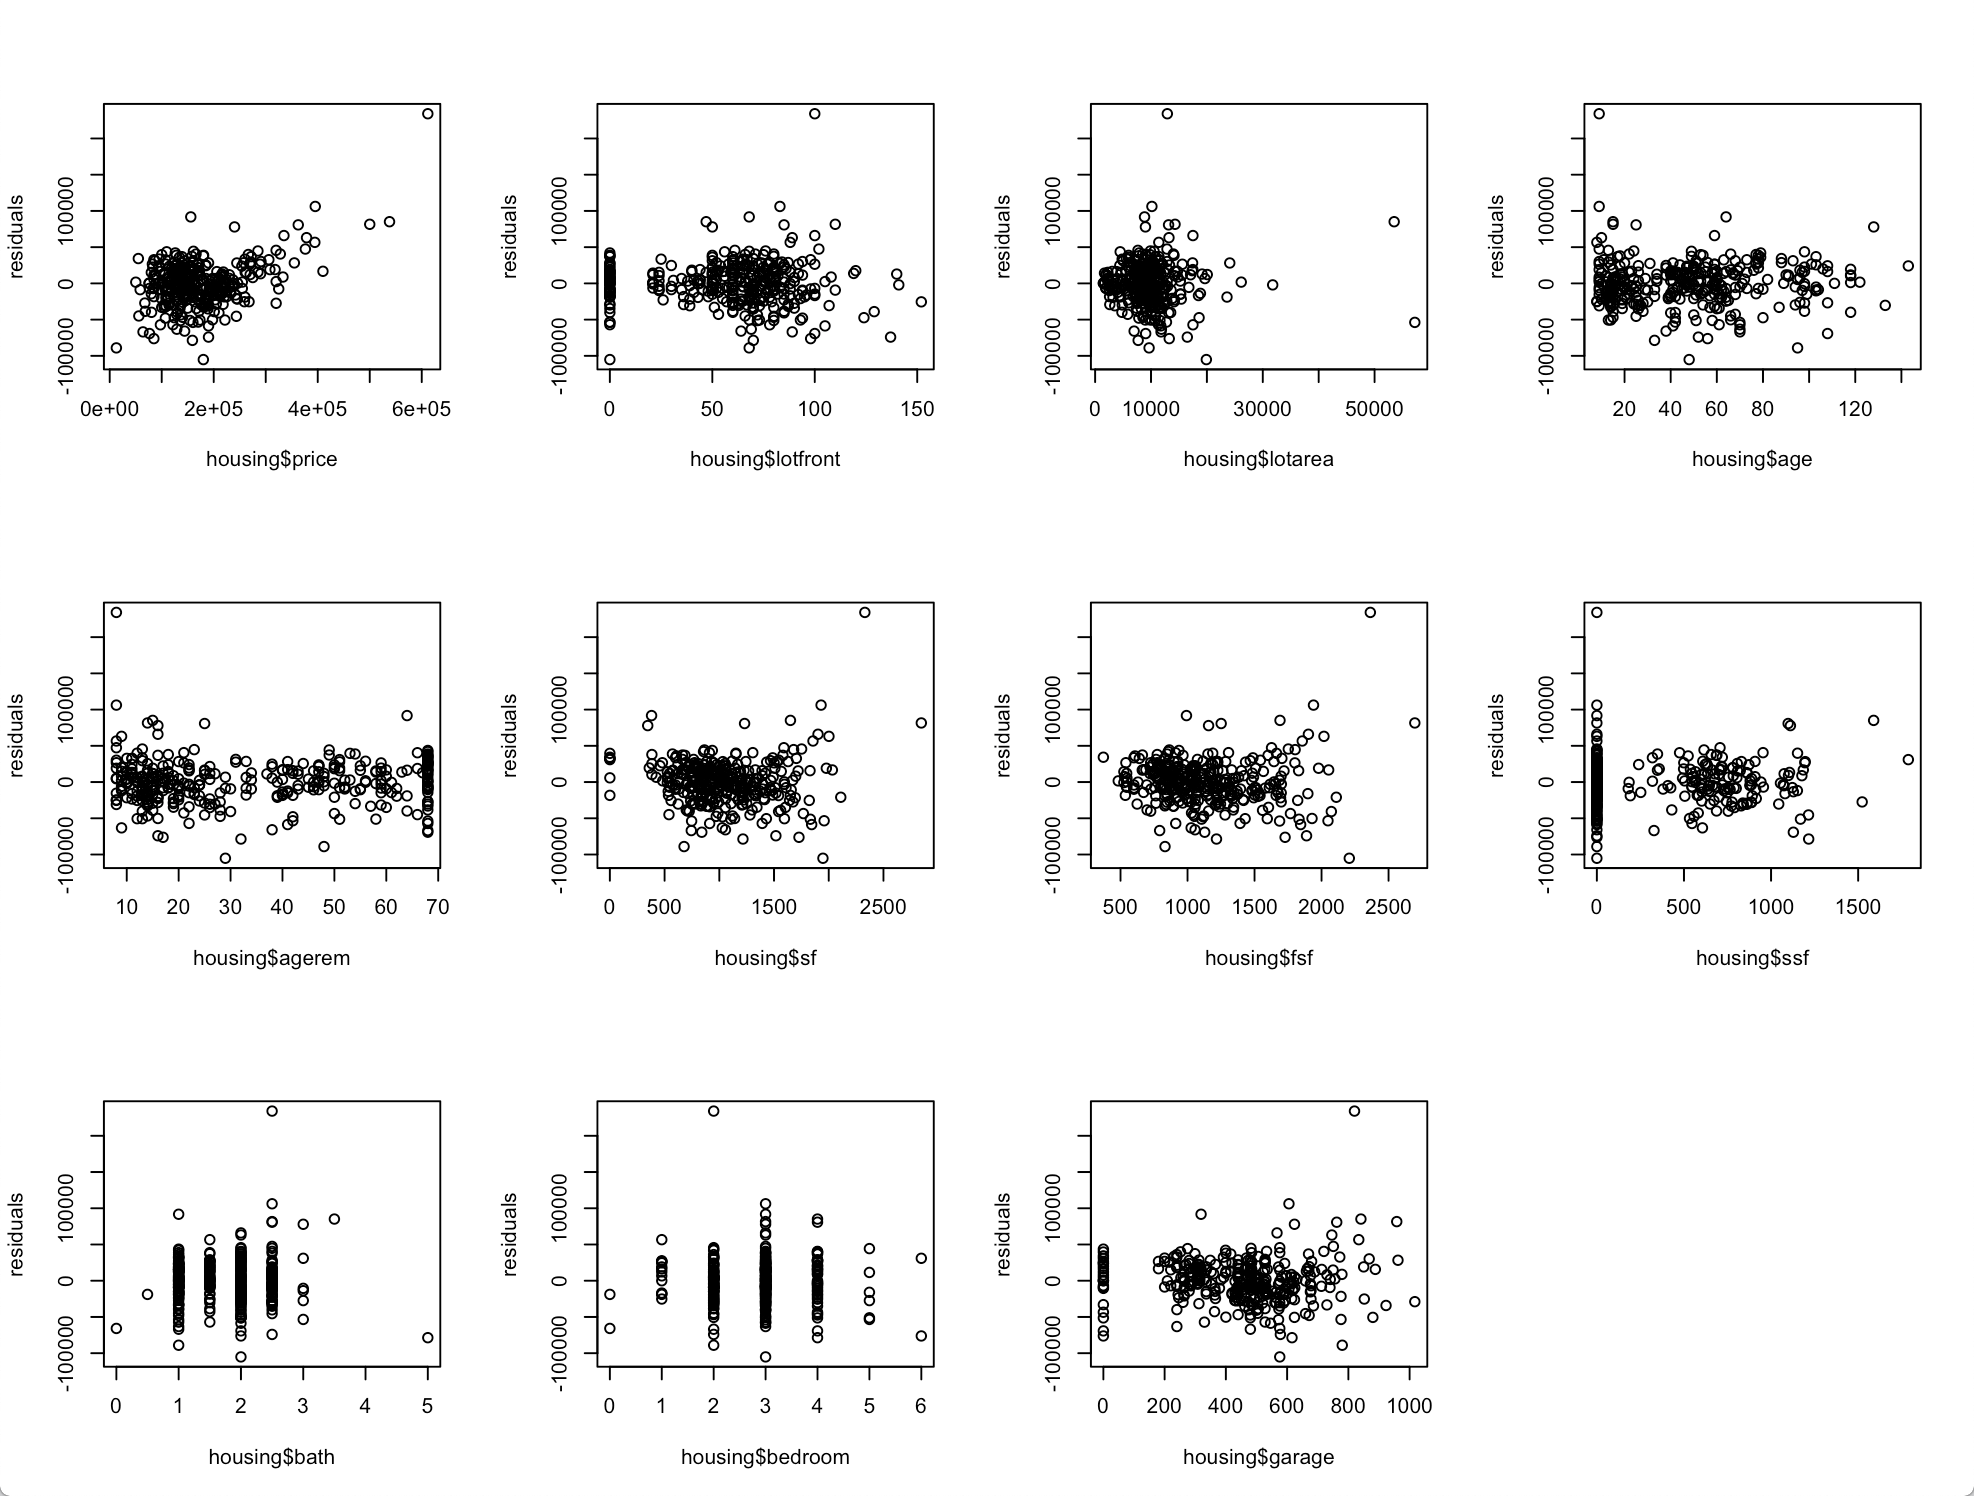
\includegraphics[scale = 0.5]{residual_plot.png} \\
By oberseve the residual plot against response variable and residual plot agianst some other predictors, we notice that most plot doesn't show up any systematically pattern. however for some plot such as residuals against lotfront and residuals against price, there seems to have some pattern. The former implies some degree of non linearity, the latter implies some degree of non-constancy of variance. Such observations give us a reason to consider more terms in our model, meanwhile we also might want remove certain terms. The model selection selection recorded our method to remove predictors and include interactions.\\
We also want our residuals in the current model follow the normal distrubution, we use QQNorm plot for checking such assumption: \\
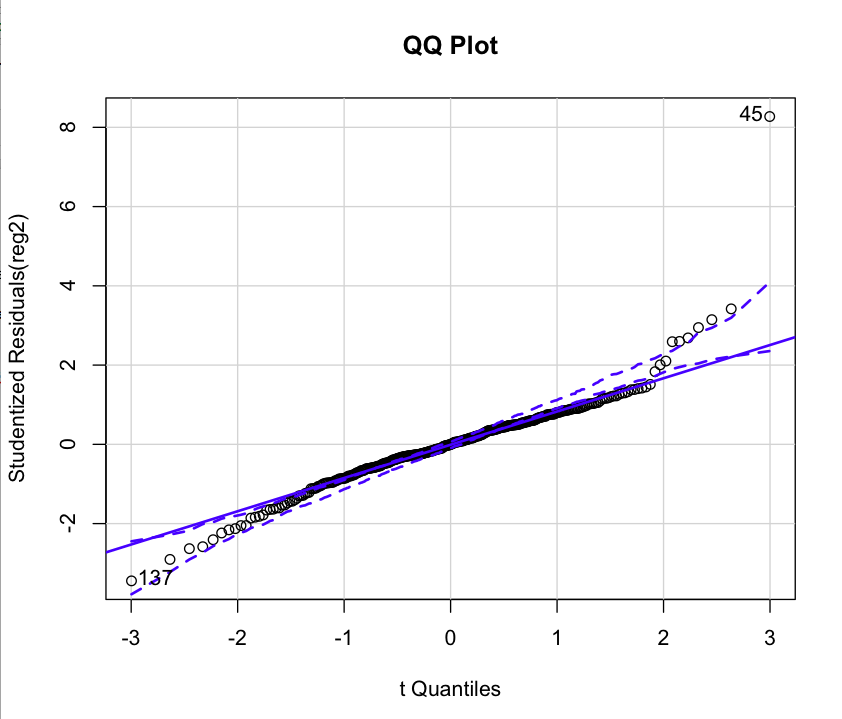
\includegraphics[scale = 0.5]{qq.png}\\
The QQ plot seems reasonably good. Hence we concluded that the residuals followed normal distribution.

\section*{Data transformations}
We didn't preprocessing data in the original first order linear model. However in latter model we added some interaction terms, we centered each predictor variables to avoid internel computational errors.

\section*{Model Selection}
We want to know if certain regression coefficients should be zero, which means weather certain predictor should be droped out from our model. We decided to use F-test with $\alpha = 0.01 $on $H_0: \beta_i = 0, H_1 \beta_i neq 0$ for each $\beta_i$. The reason we prefer F-test rather than T test is that the possible existance of muticuvlinear might affence the accuracy of T test. To achieve F test for each single coefficient, we use type 2 SS:\\
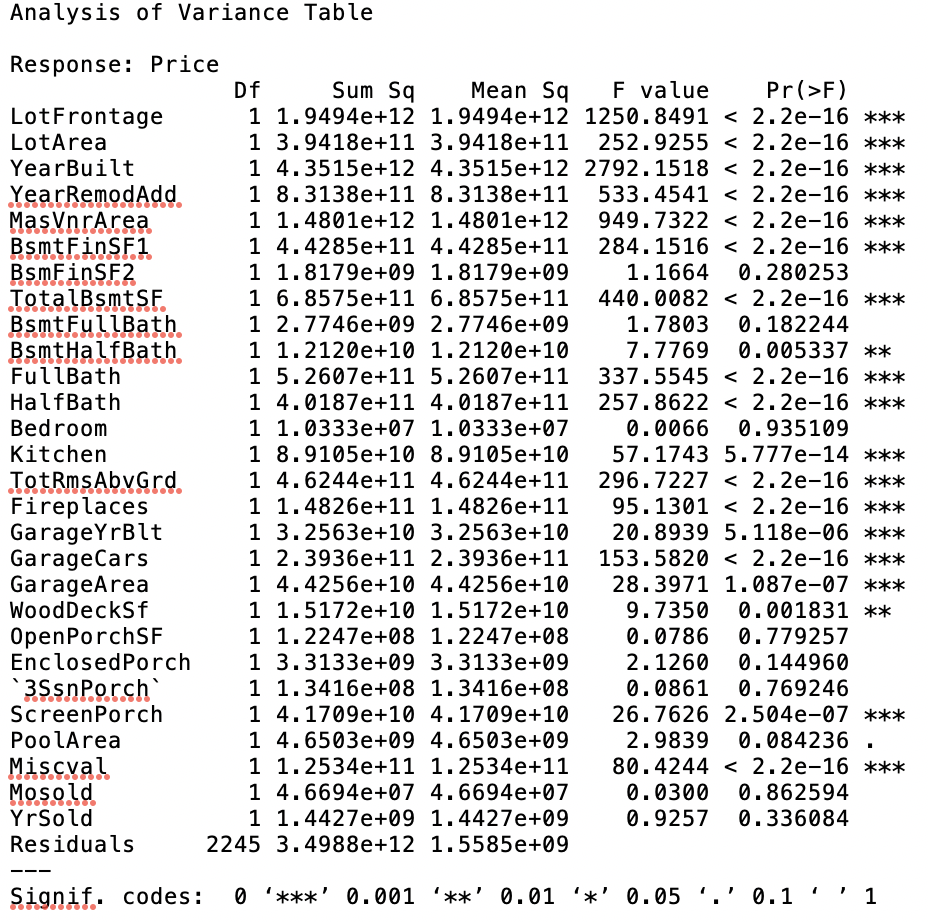
\includegraphics[scale = 0.5]{my_anova1.png} \\
From the result of the anova table, we concluded that we can actually drop out night predictors while only keeping 19 predictors.\\
Now we have a more compact model. As the residual plot implies, we are also interested in considiering the potential interaction among those 19 predictors. We first oberseved the correlation matrix of the predictors:\\
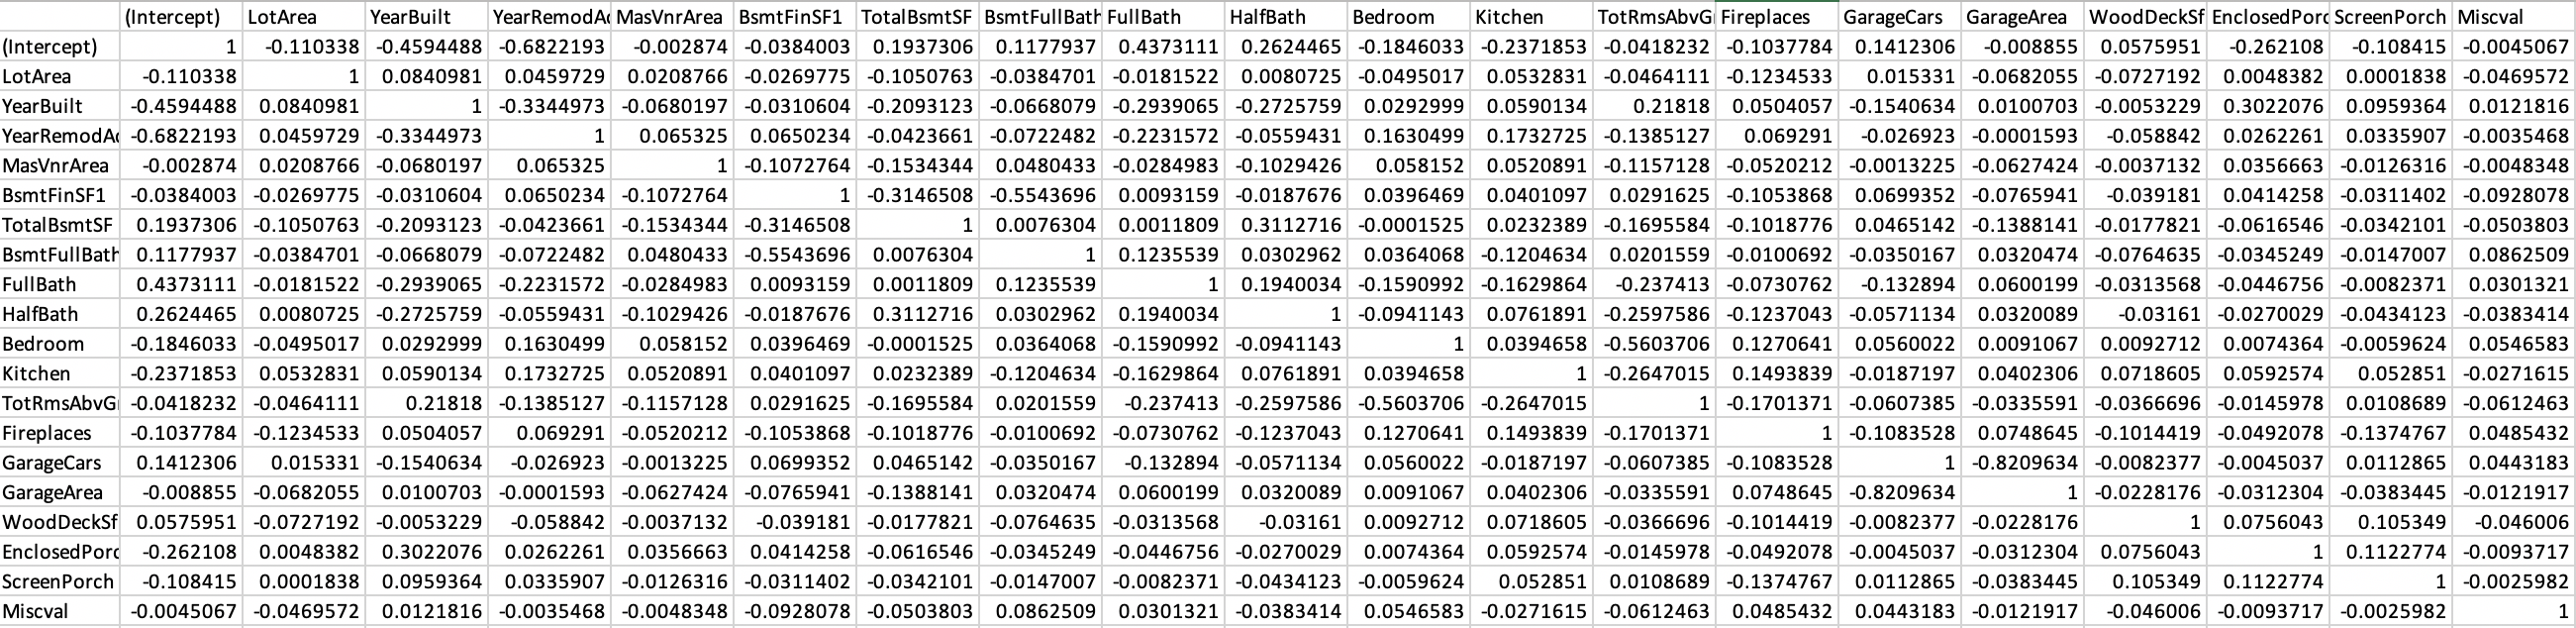
\includegraphics[scale = 0.4]{cor.png}\\
As the matric indicated there indeed exists some high correlated terms. However its infeasible to hiearchly adding all of the interaction terms in our model and test them one by one, since there are a total of 190 interaction terms. We decided to first included all interaction in our model, and drop those terms that failed to pass the F test with $\alpha = 0.01$. We first center all the predictor variables by their means to avoid some rcomputational rounding error when internelly solving inverse matrix :\\
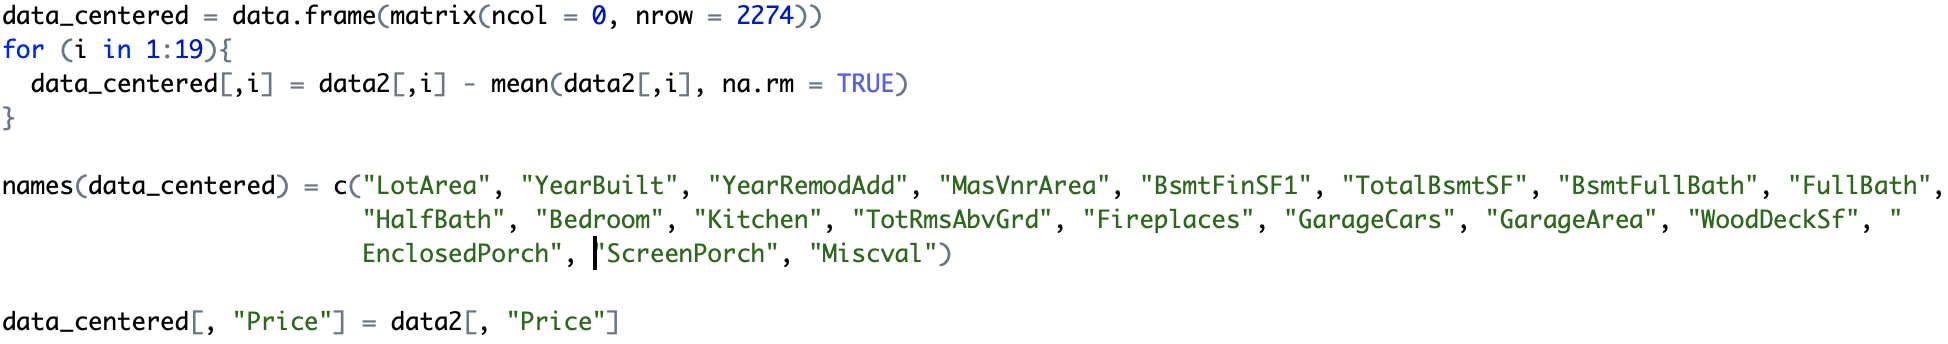
\includegraphics[scale = 0.5]{code1.png}\\
Then we fit the orignal predictors with all their pairwise interaction terms in the first order model:\\

\includegraphics[scale = 0.5]{code2.png}\\
Finally we run the deletion procedure:\\
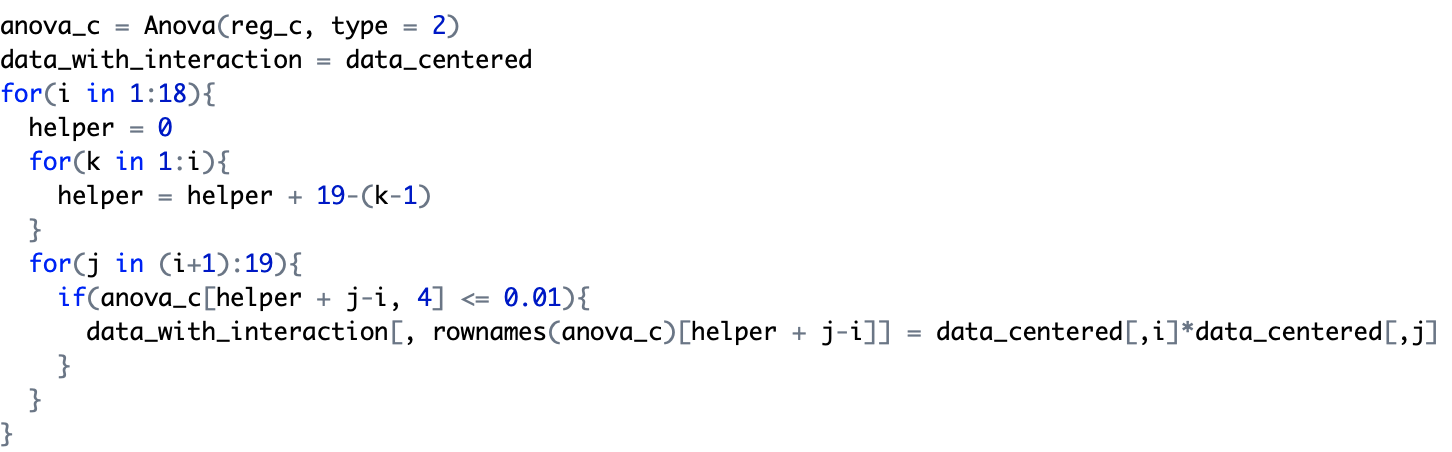
\includegraphics[scale = 0.5]{code3.png}\\
The new model summary is as follows:\\
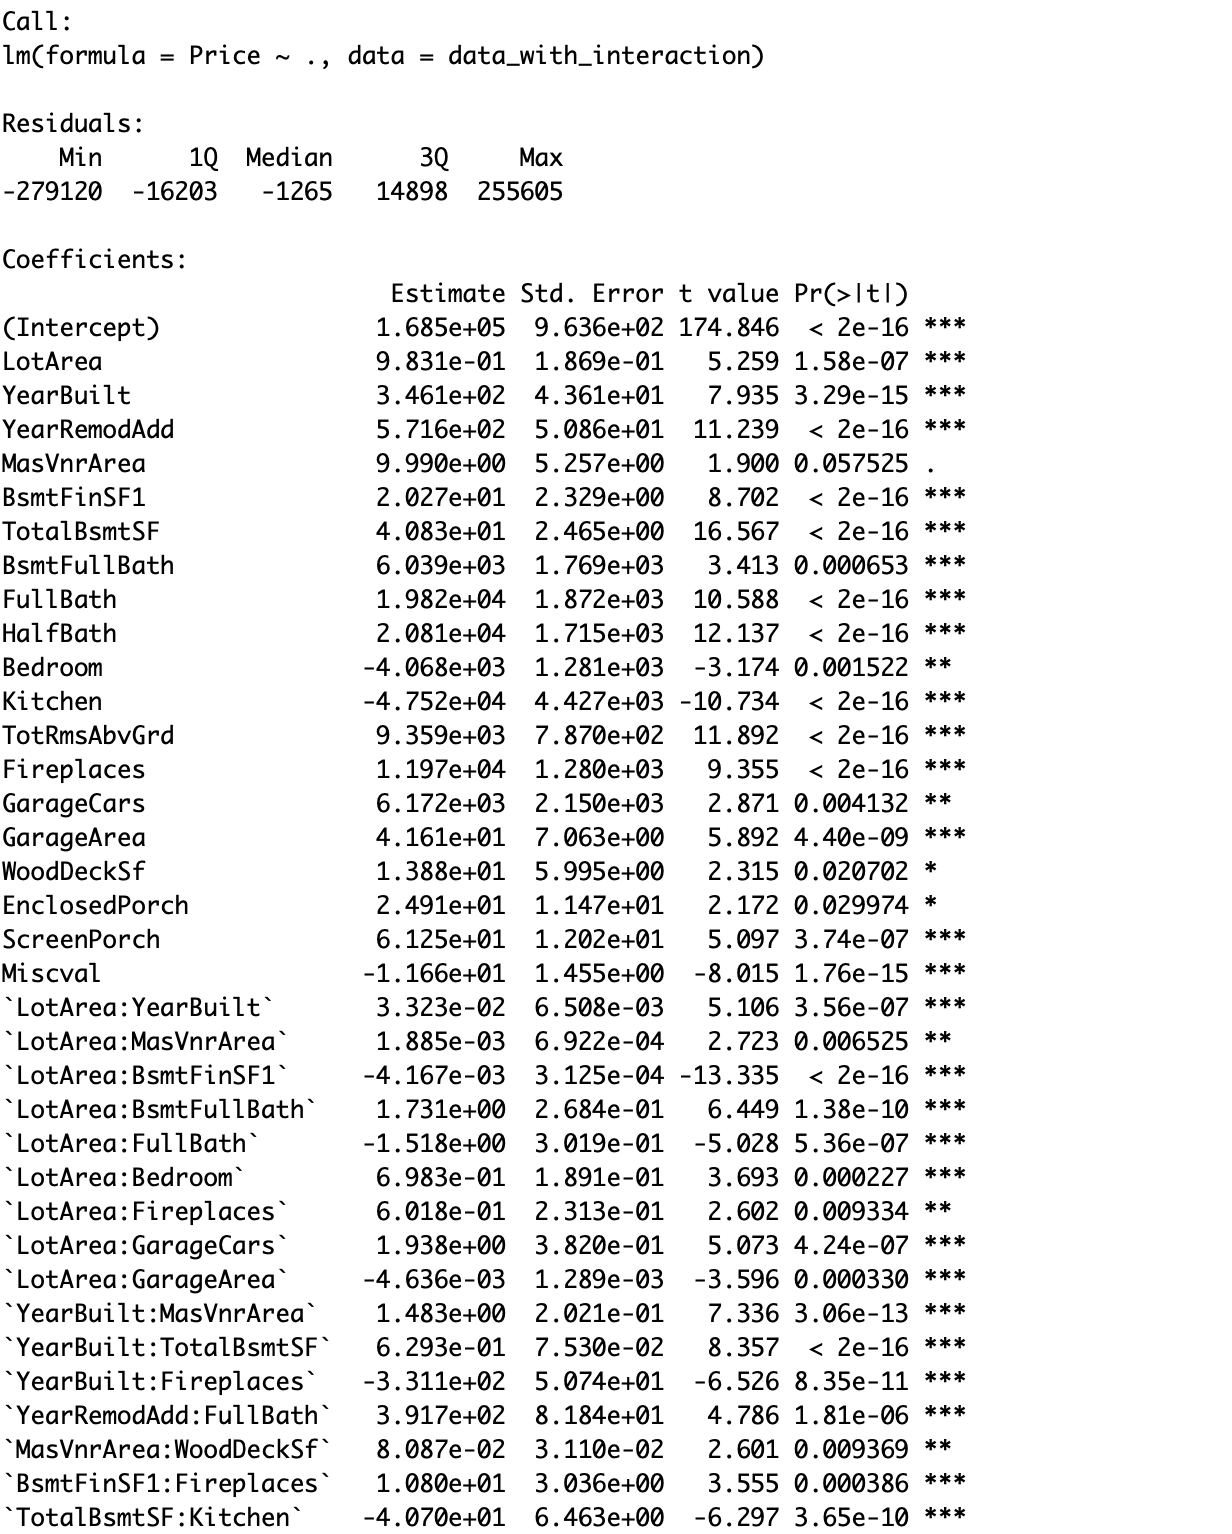
\includegraphics[scale = 0.5]{reg_f1.png}\\
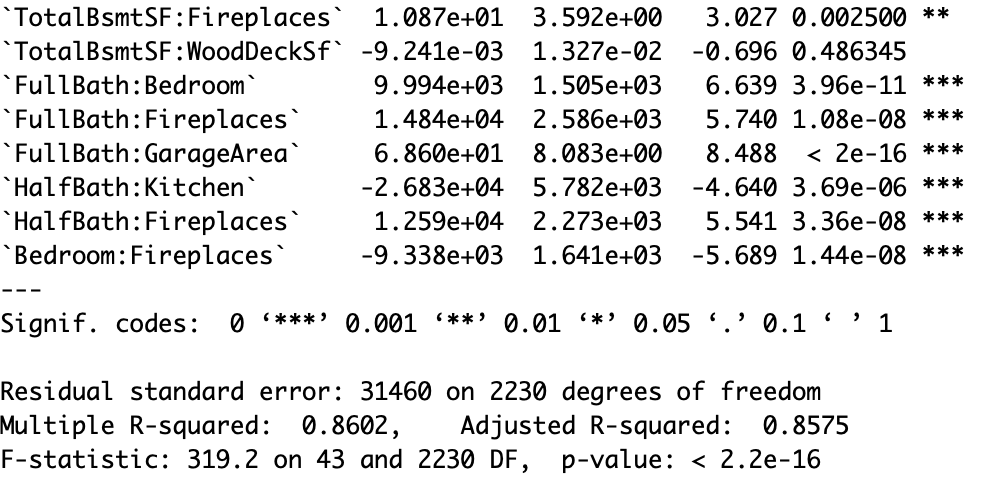
\includegraphics[scale = 0.5]{reg_f2.png}\\
By the result of F test, we droped most of the interaction terms while only keeping 24 of them. And we randomly plot around 350 observations and their corresponding three hundred fitted value, denoted by symbol "x" and "o", to visualize our model's performance:\\
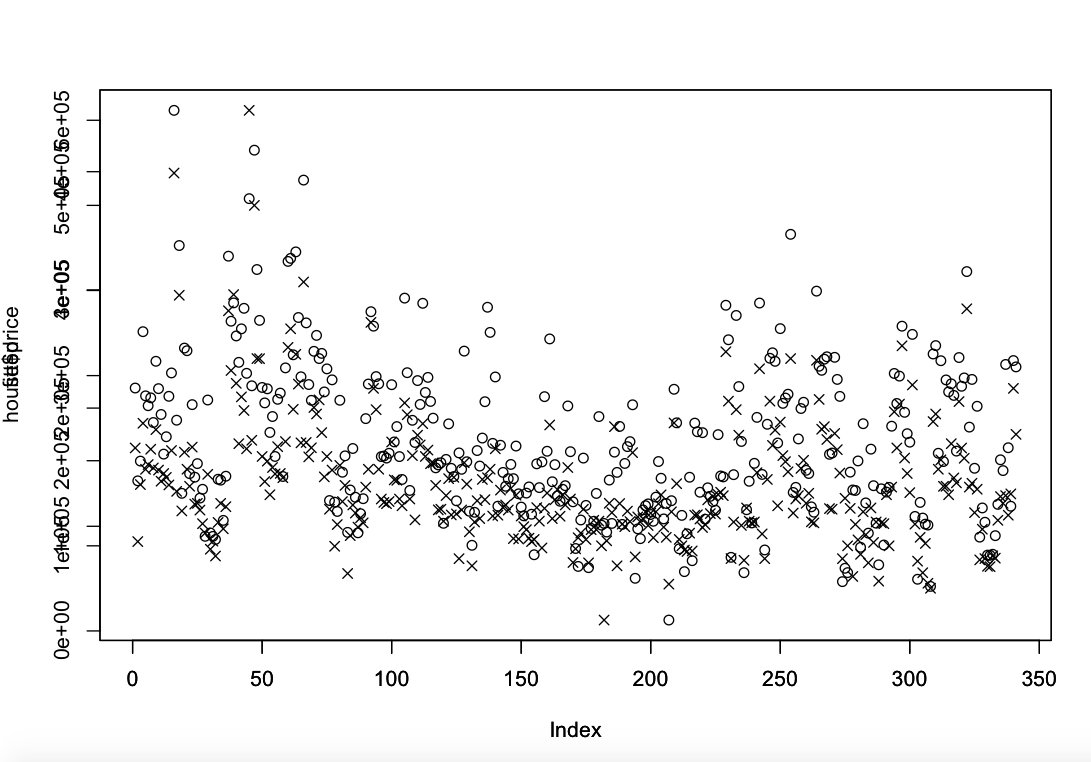
\includegraphics[scale = 0.5]{result.png}


\section*{Interpretations}
 The y-intercept for our model was estimated at \$16850 indicating that if all variables were set to zero, we expect this to be the starting price of a house. Our positive beta values show that these corresponding variables have a positive, linear relationship to housing price. If we increase these aspects, our house price is expected to increase as well. Variables with negative beta values have the opposite effect on the house price. These variables include age of the home and the years since the house has been remodeled. Housing prices will increase if they have been built or remodelled in recent years. Our r-squared value is calculated at 0.8602. This means that 82.29\% of the variability in housing prices are explained by the x-variables in our model. Although a high r-squared value does not indicates that this is a good model to estimate the price of a house, it still indicates that our model make sense in some way.\\
 By including the interaction terms, the mean square error were reduced about ten times. Although its still a considerably large number. One potential reason for might due to the distribution of the response variable is very sparse, and the range is numerically large. In selecting our model, we chose different variables that we believed would influence the pricing of homes. We put our data into R and the ANOVA table and F-test revealed that some of our original variables did not significantly contribute to our model. From here, we decided to remove this variable which led us to the model that we have presented. We chose a multiple linear regression model with interaction terms because we believed that there would be several highly influential factors in pricing a home rather than prices relying on a single variable.

\section*{Possible Problems}
The biggest problem of our dataset is that it will be most applicable to the town of Ames, Iowa. Our data was retrieved from this specific area and, therefore, is best used to estimate prices of the houses here. This would not be a good model to use for other cities that have large economic differences from Iowa. We believe that factors such as crime rate, income, etc. have a significant effect on housing prices as well, so we cannot rely on this model to give accurate estimates for houses in areas that are not similar to Ames. For example, a house price in a city, such as Boston, will have greater beta values as these houses tend to sell at higher prices than Ames, on average. Another problem that we noticed is that the beta values for number of bedrooms and kitchens is negative. We expected that the more bedrooms and bathrooms a house contains, the higher the price of the house would be. However, this was not the case in our data analysis. This is one aspect of our model that we are questioning and it may be tied with variable dependence even though we have included interaction terms. If we included more interactions and higher order terms in our model, we might achieve a better model. However a linear model with too high order suffer a lot from overfitting: It often perform well in obervation set, but perfromed poorly for new data.\\
We also delete tens of categorical variables from original dataset, which might also leads problem. Those categorical variables might be the key for having a good model.\\
The other major problems is that a fitness of a overall linear model remain questionaire. In the persepective of predicting, there might be the model that perform much better than linear model, such as decision tree or neural network... Or even adding $l_1$ or $l_2$ regularizations to linear model might make it perfrom much better. 

\section*{Conclusion}
Overall our linear regression model had some problems and it was not perfect but it should work as a game model to estimate housing prices. It cal be a useful tool in helping individuals find a house that is fitting for their budget. We can alter different aspects of our dream home and find the perfect combination that work best with our needsand wallets. Overall, linear model overperfrom many other model such as decision trees, in the persepective of interpretation. By our interpretation among interaction terms, we obtain a lot of useful information that might reveal the potential relashionship of response variables and predictors.





\end{document}